\documentclass[a4paper, 12pts]{amsart}

\usepackage[utf8]{inputenc}
\usepackage{listings}
\usepackage{datetime}
\usepackage{tikz}
\usetikzlibrary{arrows}

\newdateformat{monthyeardate}{
  \monthname[\THEMONTH], \THEYEAR}

\title{Different to the Minimizing Function on Neural Networks}
\author{Andrés Felipe Ortega Montoya\\
  \monthyeardate{\today}}

\begin{document}
\maketitle
\tableofcontents
\section{Basics on Neural Networks}
A neural network can be viewed as a directed graph in which each vertex serves
as a ``neuron'' and have an associated output value for how active it is.
For the first layer of neurons, their output values are simply input given to
the network. In the case of other neurons it will calculated taking into
account the activation values of all neurons connected to it. The output or
``return'' value of the neural network will be how active are all the neurons
that have no connections, or the ones belonging to the output layer. It is
common to have a set of intermediate neurons between the input and output layer
in order to give the network the capability of more complex tasks.

\begin{figure}[!h]
  \centering
  \def\layersep{2.5cm}

  \begin{tikzpicture}[shorten >=1pt,->,draw=black!50, node distance=\layersep]
    \tikzstyle{every pin edge}=[<-,shorten <=1pt]
    \tikzstyle{neuron}=[circle,draw,minimum size=17pt,inner sep=0pt]
    \tikzstyle{annot} = [text width=4em, text centered]

    % Draw the input layer nodes
    \foreach \y in {1,...,4}
    % This is the same as writing \foreach \name / \y in {1/1,2/2,3/3,4/4}
    \node[neuron, pin=left:$x_\y$] (I-\y) at (0,-\y) {};

    % Draw the hidden layer nodes
    \foreach \y in {1,...,5}
    \path[yshift=0.5cm]
    node[neuron] (H-\y) at (\layersep,-\y cm) {};

    % Draw the output layer node
    \node[neuron,pin={[pin edge={->}]right:Output}, right of=H-3] (O) {};

    % Connect every node in the input layer with every node in the
    % hidden layer.
    \foreach \source in {1,...,4}
    \foreach \dest in {1,...,5}
    \path (I-\source) edge (H-\dest);

    % Connect every node in the hidden layer with the output layer
    \foreach \source in {1,...,5}
    \path (H-\source) edge (O);

    % Annotate the layers
    \node[annot,above of=H-1, node distance=1cm] (hl) {Hidden layer};
    \node[annot,left of=hl] {Input layer};
    \node[annot,right of=hl] {Output layer};
  \end{tikzpicture}
  \caption{Example of a neural network}
\end{figure}
\begin{figure}[!h]
  \centering
  \def\layersep{2.5cm}

  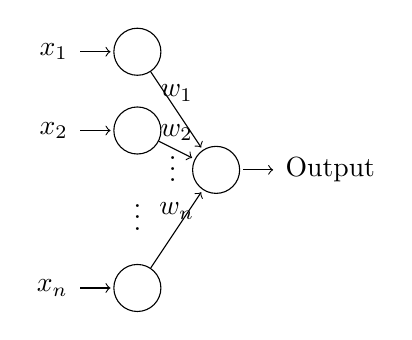
\begin{tikzpicture}[shorten >=1pt,->, node distance=\layersep]
    \tikzstyle{every pin edge}=[<-,shorten <=1pt]
    \tikzstyle{neuron}=[circle,draw,minimum size=17pt,text height=.5ex,
    inner sep=1pt]

    \node[neuron, pin=left:$x_1$] (I-1) at (0,-1) {};
    \node[neuron, pin=left:$x_2$] (I-2) at (0,-2) {};
    \node (D) at (0,-3) {$\vdots$};
    \node[neuron, pin=left:$x_n$] (I-n) at (0,-4) {};
    
    \node[neuron,pin={[pin edge={->}]right:Output}] (O) at (\layersep,-2.5) {};

    \path (I-1) edge node [above] {$w_1$} (O)
          (I-2) edge node [above] {$w_2$} (O)
          (D)   edge [draw=none] node [above] {$\vdots$} (O)
          (I-n) edge node [above] {$w_n$} (O);

  \end{tikzpicture}
  \caption{Example of a neural network}
\end{figure}

\end{document}
